%\begin{filecontents*}{example.eps}
%!PS-Adobe-3.0 EPSF-3.0
%%BoundingBox: 19 19 221 221
%%CreationDate: Mon Sep 29 1997
%%Creator: programmed by hand (JK)
%%EndComments

%\end{filecontents*}
%
%\documentclass{svjour3}                     % onecolumn (standard format)
%\documentclass[smallcondensed]{svjour3}     % onecolumn (ditto)
\documentclass[12pt,oneside,a4paper]{article}  

\usepackage{apacite}
\usepackage{appendix}
\usepackage{amsmath}
\usepackage{amsthm}
\usepackage{tikz}
\usepackage{amssymb} % for approx greater than
\usepackage{caption}
\usepackage{subcaption}
\usepackage{placeins} % for \FloatBarrier
\usepackage{graphicx}
%\usepackage{subcaption}
\usepackage{longtable}
\usepackage{setspace}
\usepackage{booktabs}
\usepackage{tabularx}
\usepackage{subfig}
\usepackage{xcolor,colortbl}
\usepackage{chngpage}
\usepackage{natbib}
\bibpunct{(}{)}{,}{a}{}{;} 
\usepackage{url}
\usepackage{nth}
\usepackage{authblk}
\usepackage[most]{tcolorbox}
\usepackage[normalem]{ulem}
\usepackage{amsfonts}

% columns for longtable
%\usepackage{arydshln} % Dashed lines in matrices

\usepackage[margin=1in]{geometry}
%\doublespacing % for review

% line numbers to make review easier
%\usepackage{lineno}
%\linenumbers

%\usepackage{soul}% for \st{}

%%%%%%%%%%%%%%%%%%%%%%%%%%%%%%%%%%%%%%%%%%%%%%%%%%%%%%%%%%%%%%%%%%%%%%%%%%%%%%
% for section 4 math environments
%\theoremstyle{definition}
%\newtheorem{definition}{Definition}[section]
%\newtheorem{theorem}{Theorem}[section]
%\newtheorem{proposition}{Proposition}[section]
%\newtheorem{corollary}{Corollary}[proposition]
%\newtheorem{remark}{Remark}[section]
%
%%%%%%%%%%%%%%%%%%%%%%%%%%%%%%%%%%%%%%%%%%%%%%%%%%%%%%%%%%%%%%%%%%%%%%%%%%%%%%
%\begin{filecontents*}{example.eps}
%!PS-Adobe-3.0 EPSF-3.0
%%BoundingBox: 19 19 221 221
%%CreationDate: Mon Sep 29 1997
%%Creator: programmed by hand (JK)
%%EndComments
%gsave
%newpath
%  20 20 moveto
%  20 220 lineto
%  220 220 lineto
%  220 20 lineto
%closepath
%2 setlinewidth
%gsave
%  .4 setgray fill
%grestore
%stroke
%grestore
%\end{filecontents*}
%\RequirePackage{fix-cm}

\newcommand\ackn[1]{%
  \begingroup
  \renewcommand\thefootnote{}\footnote{#1}%
  \addtocounter{footnote}{-1}%
  \endgroup
}

% Affiliations in small font size
%\renewcommand\Affilfont{\small}
\newcommand{\absdiv}[1]{%
  \par\addvspace{.5\baselineskip}% adjust to suit
  \noindent\textbf{#1}\quad\ignorespaces
}
\newcommand{\rd}[1]{\textcolor{red}{#1}}
%\defcitealias{HMD}{HMD 2016}

\begin{document}


\title{Trends in United States life expectancy and disability above age 50: Delayed onset, improved recovery, mortality change, or compositional change?}

\author[1]{Tim Riffe\thanks{riffe@demogr.mpg.de}}
\author[2]{Neil Mehta}
\author[1]{Daniel Schneider}
\author[1,3]{Mikko Myrskyl\"a}

\affil[1]{Max Planck Institute for Demographic Research}
\affil[2]{University of Michigan, Ann Arbor}
\affil[3]{University of Helsinki}

%\authorrunning{Short form of author list} % if too long for running head

%\institute{   Tim Riffe \at
%              Max Planck Institute for Demographic Research.
%              Konrad-Zuse-Str. 1. 18057 Rostock, Germany\\
%              \email{riffe@demogr.mpg.de}\\
%              Tel.:  +49 176 232 858 45\\
%              Fax: +49 381 2081 - 280
%\and 
% Neil Mehta \at
%              Department of Health Management and Policy. 
%School of Public Health.
%M3531 SPH II
%Ann Arbor, MI 48109-2029\\
%              \email{nkmehta@umich.edu }
%\and
%Daniel Schneider \at
%              Max Planck Institute for Demographic Research.
%              Konrad-Zuse-Str. 1. 18057 Rostock, Germany\\
%              \email{schneider@demogr.mpg.de}      
%\and
%Mikko Myrskyl\"a \at
%              Max Planck Institute for Demographic Research.
%              Konrad-Zuse-Str. 1. 18057 Rostock, Germany\\
%              \email{myrskyla@demogr.mpg.de}   
%              }
%              
%

\maketitle

\vspace{-2em}

\begin{abstract}
\absdiv{Background} 
Life expectancy and disability free life expectancy at older ages in the United States has steadily
increased in recent decades. We do not know whether changes in
disease onset, recovery, or mortality or compositional change drives this trend.
\absdiv{Objective}
We aim to determine how much of the change in
life expectancy between 1995 and 2015 is due to changes in onset, recovery,
mortality, as well as changes SES composition coupled with SES gradients in disability and mortality.
\absdiv{Data and Methods}
We use the US Health and Retirement Study to estimate transition probabilities between disability
states, as well as state-specific death probabilities, for the years 1996,
2006, and 2014. We calculate remaining disability free, disabled, and total life
expectancy at age 50 using multistate Markov matrix models. We decompose the change in expectancies
 into components for onset, recovery, mortality, and compositional effects using pseudo-continuous decomposition.
\absdiv{Results}
We describe preliminary results for males and females.
Perhaps counter to intuition, most change in disability free life expectancy is due to
mortality and not to onset of or recovery from disability. Most of the two-year
increase in disability free life expectancy for males since 1996 is due to decreased mortality of both disabled and disability free states, whereas delayed onset and slowed recovery from disability offset each other. Females have undergone a disability expansion, driven largely by deterioration in recovery rates since 2006.

\absdiv{Conclusions}
Secular mortality change has been the main driver of mean time spent free of and in disability. Potential improvement in disability recovery rates is a strong lever to both increase overall life expectancy and shift years lived in disability to good health. Life expectancy improvement at age 50 from educational expansion has been modest in the period studied, but holds much potential to fuel further increases in life expectancy for both males and females.
\end{abstract}

[\rd{NOTE:} This is a work in progress, and values may change as we continue experimentation with transition probability estimation and state spaces. After many specifications at this stage the main story has not changed--- we're just iterating toward better transition probabilities.]

\section{Introduction}
The USA has fallen behind in the rankings of life expectancy compared with other high income countries. Although this well-known finding is primarily due to mortality differences in young and middle ages, the USA has also lost ground in rankings of life expectancy in older ages \citep{HMD}. Figure~\ref{fig:uslose} displays trends in remaining life expectancy at age 50 among all high-income HMD countries with data in both 1996 and 2014, and it shows the USA to be under-performing--- This picture motivates our work. The USA had already dropped to a modest ranking by 1996 (\nth{17} of 23 for females and \nth{11} of 23 for males), but by the year 2014 the rank position had deteriorated to last and penultimate for females and males, respectively. Life expectancy in older ages has in plain terms stagnated since 2010. 

\begin{figure}[ht!]
\centering
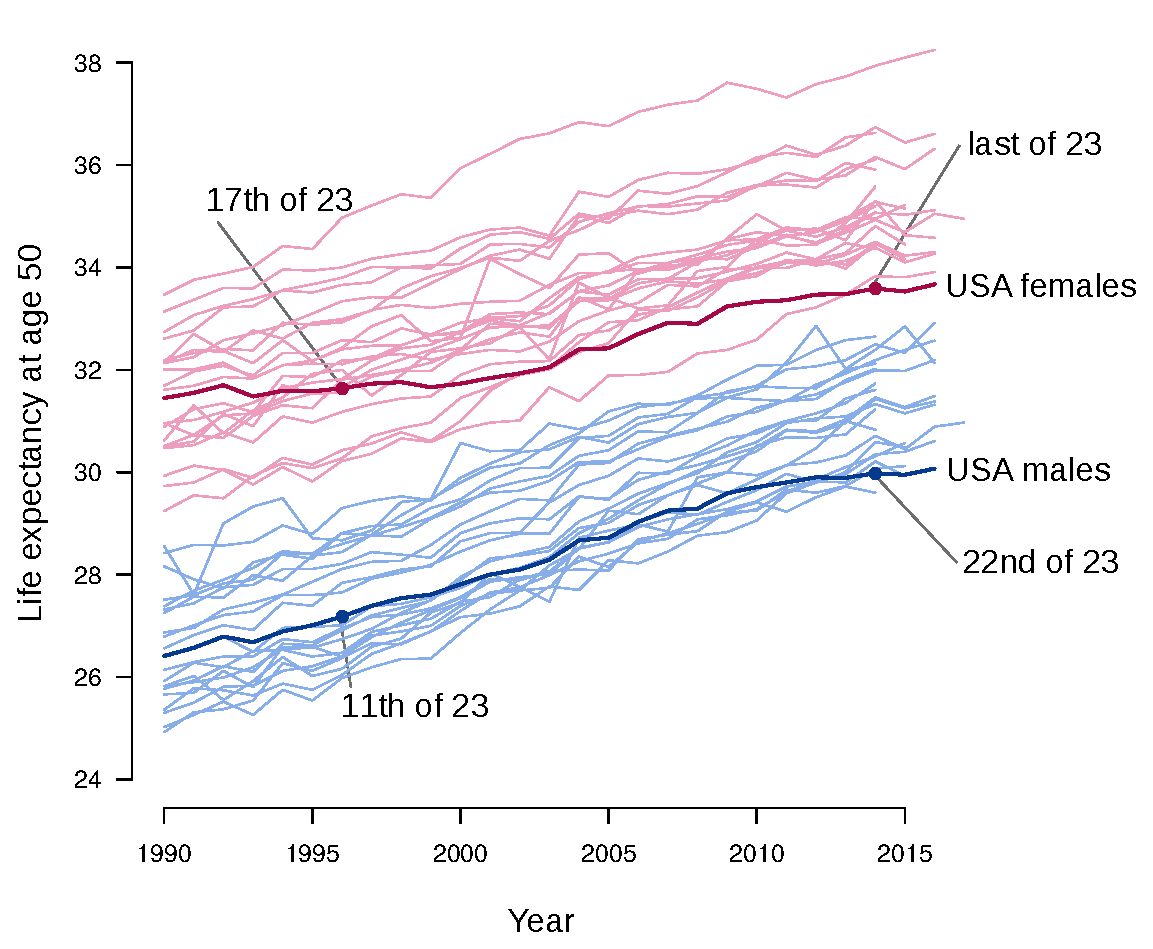
\includegraphics[scale=.7]{Figures/USAvsOthers_Ink.pdf}
\caption{Trends in male and female remaining life expectancy at age 50 from 1990 to 2016 in 23 high-income HMD countries:  \\ \footnotesize Australia, Austria, Belgium, Switzerland, Germany, Denmark, Spain, Finland, France, Ireland, Israel, Italy, Japan, Luxembourg, the Netherlands, Norway, Portugal, Sweden, Taiwan, Great Britain, and the United States. We exclude countries of the contemporary Eastern European mortality pattern, as well as HMD countries without data for the years 1996 and 2014.}
\label{fig:uslose}
\end{figure}

Mean remaining lifespan at age 50 in the USA increased by 2.9 years for males and 2.0 years for females in the two decades from 1996 to 2016, amounting to 10\% and 6\% increases, respectively. In the net, mortality has improved over this period. Despite under-performance in international perspective, there is still some success to account for. Several factors underlie this modest improvement, including improved living standards and nutrition over the lifecourse of the cohorts composing the 50+ population, as well as medical improvements allowing for quicker and more certain recovery from many health conditions. Cures, lifesaving, and life-extending treatments may delay the deaths of both healthy and chronically ill or disabled persons, and therefore may contribute to increasing both years lived in a state of morbidity and in good health. For the typical case of population-level death rates that underlie estimates of period life expectancy, it is not clear whether a rate improvement comes about due to improvements in the health and well-being of a population, the effects of medicine, or the population composition with respect to various kinds of risk sets, such as the educational composition. 

Our objective is to quantify how much of the increase in life expectancy (LE), disabled life expectancy (DLE), and disability-free life expectancy (DFLE) at age 50 is due to 1) changes in the mortality rates of the disabled and disability-free, 2) changes in SES-differential mortality, as captured by education-specific mortality, 3) changes in the fraction in each educational group and the education-specific prevalence of disability of those entering the 50+ population, and 4) changes in the onset of disability (disablement) and recovery from disability in old ages. These effects can be condensed as mortality change, versus disability change, versus compositional change. We consider this question to be of great importance because results will reveal the most important levers in life expectancy change, and these components in turn may indicate the potential for future improvements, but also the culprits of contemporary stagnation. 

The present work is the only instance that we are aware of to directly decompose changes in LE, DFLE, and DLE into effects attributable to the transitions defined in a Markov process model of disability as well as the changing composition (in terms of disability and education) of newcomers to the 50+ population. Other studies have done similar decomposition exercises based on Sullivan-style healthy life expectancy \citep[e.g.,][]{andreev2003health, nusselder2005contribution, van2011contribution, heijink2011decomposing, van2013gender, freedman2016disability, chernew2016understanding}, but in these studies no account is made of differential mortality by health status or the potentially countervailing effects of onset versus recovery from disability. The literature includes good examples of incidence-based models of healthy life expectancy similar to our own \citep[e.g.,][]{crimmins2009change, reuser2011higher, montez2014cumulative}, but these have not been decomposed in the traditional demographic sense. More often, differences in transition probabilities are directly reported, or else the leverage on expectancy of individual transition probabilities is gauged on the basis of leave-one-out counter-factual exercises, simulation, or approximated analytically with sensitivity analyses \citep{reuser2010effect}.

In section~\ref{sec:methods} we briefly describe the data and methods used to answer our main questions. In section~\ref{sec:results} we describe trends in LE, DLE, and DFLE at age 50, and we decompose changes over time in each of these expectancies into effects from changes in the onset of disablement, recovery, mortality with and without disability, and changes in the educational composition and education-specific disability prevalence at age 50. In section~\ref{sec:discussion} we formalize what can be learned from this analysis, how it relates to the literature, and the limitations of our data and research design. We conclude with recommendations for further scientific inquiry and for population-level health intervention.

\section{Methods and materials}
\label{sec:methods}
% verbrugge ADL progression could be used as proxy for mild and severe
We estimate disability free and disabled life expectancy using incidence-based discrete-time Markov models. The model separates the population into two groups: disability free and disabled, where disability is defined as having at least one of a set of 5 activities of daily living (ADLs) \footnote{The five ADLs include bathing, eating, dressing, walking across a room, and getting into or out of bed.}. Fig.~\ref{fig:statespace} shows the formal state space used in our model of disability. We use RAND version P of the US Health and Retirement Study \citep{RAND, HRS} to estimate the probability of transitioning into and out of disability, and the probability of dying with and without disability with multinomial logit models. We stratify models by sex and three educational attainment categories\footnote{Education categories include 1) less than high school, 2) high school, including GED and some college, but no degree, and 3) university degree, including 2-year associates degrees.}, and control for four race and ethnicity categories \footnote{}. Age-effects for two-year age groups from age 50 to 110 (31 age groups) are captured flexibly with splines.\footnote{We use 2-year age groups because HRS waves are spaced two years apart.} With this we obtain point estimates for transition probabilities in the years 1996, 2006, and 2014. 

\begin{figure}[ht!]\centering
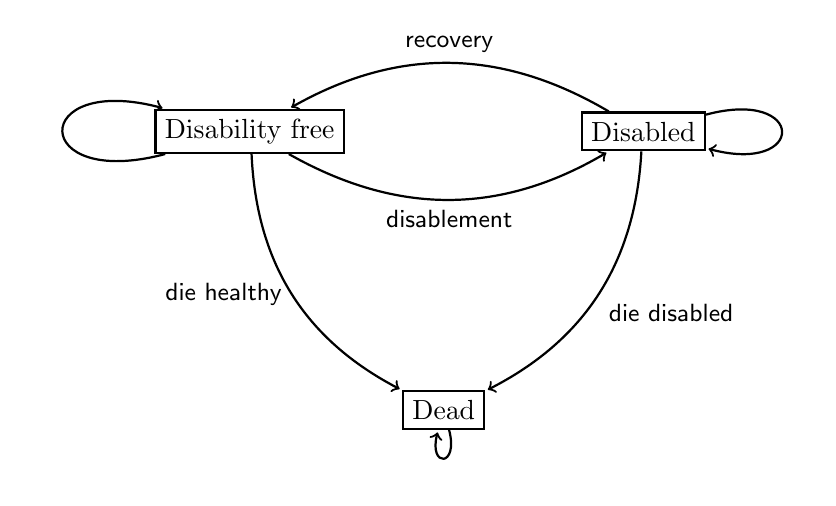
\begin{tikzpicture}[->,shorten >=1pt,auto,node distance=5cm,
  thick,main node/.style={draw}]

  \node[main node] (1) {Disability free};
  \node[main node] (2) [right of=1] {Disabled};
  \node[main node] (3) [below left of=2,xshift=1cm] {Dead};

  \path[every node/.style={font=\sffamily\small}]
    (1) edge [bend right] node [left] {die healthy} (3)
    (1) edge [bend right] node [below] {disablement} (2)
    (1) edge [loop left] node {} (1)
    (2) edge [bend right] node [above] {recovery} (1)
    (2) edge [loop right] node {} (2)
    (2) edge [bend left] node {die disabled} (3)
    (3) edge [loop below] node {} (3);
    
\end{tikzpicture}\\

\caption{State space used for our discrete Markov model. Disabled is defined as having at least one (of a set of five) ADLs. Age transitions are not depicted in the diagram for simplicity. We assume no transitions between education states after age 50, and therefore this is the state space for any given education group.}\label{fig:statespace}
\end{figure}

Given age schedules of transition probabilities depicted in Fig~\ref{fig:statespace} for each educational group and year, as well as the prevalence of disability at age 50 for each educational group and the fraction of the population in each group, the calculation of life expectancy follows a well-known set of matrix calculation steps, which we omit for the sake of brevity. These steps can be captured in a single function, $e^i(\textbf{p},\pi)$, where $e^i()$ defines the average time spent in the $i^{th}$ state (LE, DFLE, or DLE) given a vector of age- and education-specific transition probabilities $\textbf{p}$, and a vector $\pi$ of the fraction of persons aged 50 in each educational group and disability state.\footnote{For a given year and sex, $\textbf{p}$ is of length 744: 31 age groups $\times$ 3 education groups $\times$ 2 states $\times$ 4 transition types. $\pi$ is of length 6: the fraction of the population at age 50 in 2 states $\times$ 3 education groups.} This functional form facilitates classic demographic decomposition of the change in LE, DFLE, or DLE between two time points (1996 to 2006 and 2006 to 2014) that is due to each element of $\textbf{p}$ and $\pi$. 

We decompose changes over time using the method proposed by \citet{horiuchi2008}, which is general enough and sufficiently stable for our needs and is available in the \texttt{DemoDecomp} \texttt{R} package \citep{DemoDecomp}\footnote{Other options to decompose would be to use the algorithm of step-wise replacement proposed by \citet{andreev2002algorithm}, or by carrying out a lifetable response experiment as proposed by \citet{caswell1989analysis}. The first is equally general and straightforward to set up, but it is sensitive to the order in which elements are replaced, and it does not maintain the identity $p(stay) + p(entry) + p(exit) = 1$ over the algorithm steps. The second is (we conjecture) asymptotically equivalent to the Horiuchi method, but it requires extensive matrix derivations.}. Decomposition produces an estimate of the contribution of each age-specific difference in transition probability and age-50 population fractions (by education and disability state), for a total of $744 + 6 = 750$ elements. These contributions are given in year-units, and we aggregate them in various ways to determine the degree to which changes in each transition type (each edge in the Fig.~\ref{fig:statespace} graph), as well as changes in the prevalence and educational composition of the age-50 population.

[Notes] Confidence intervals on expectancies and decomposition results will come in a later revision of this work. We may consider alternative state space definitions, and change some details with age splines. We may also estimate transition probabilities for each year in order to provide a more detailed time series. 

\section{Results}
\label{sec:results}
\subsection{Transition probabilities and life expectancy}
The transition probabilities for females in the year 2006 are given as an example to show the basic characteristics of each age pattern. These are different for each time point, education group, and between the sexes, but the basic schematic shape of each curve is essentially the same for all subgroups: i) mortality increases monotonically for both the disabled and the non-disabled, but is higher for the disabled ii) the probability of staying healthy decreases monotonically after age 50, iii) the probability of staying disabled either remains flat until near the modal age at death, after which it falls, or else it monotonically falls over all ages, iv) the probability of recovering from disability monotonically falls, and v) the probability of entering into a state of disability first increases strongly, then decreases after age 100 as the force of mortality becomes the dominant transition. 

\begin{figure}[ht!]
\centering
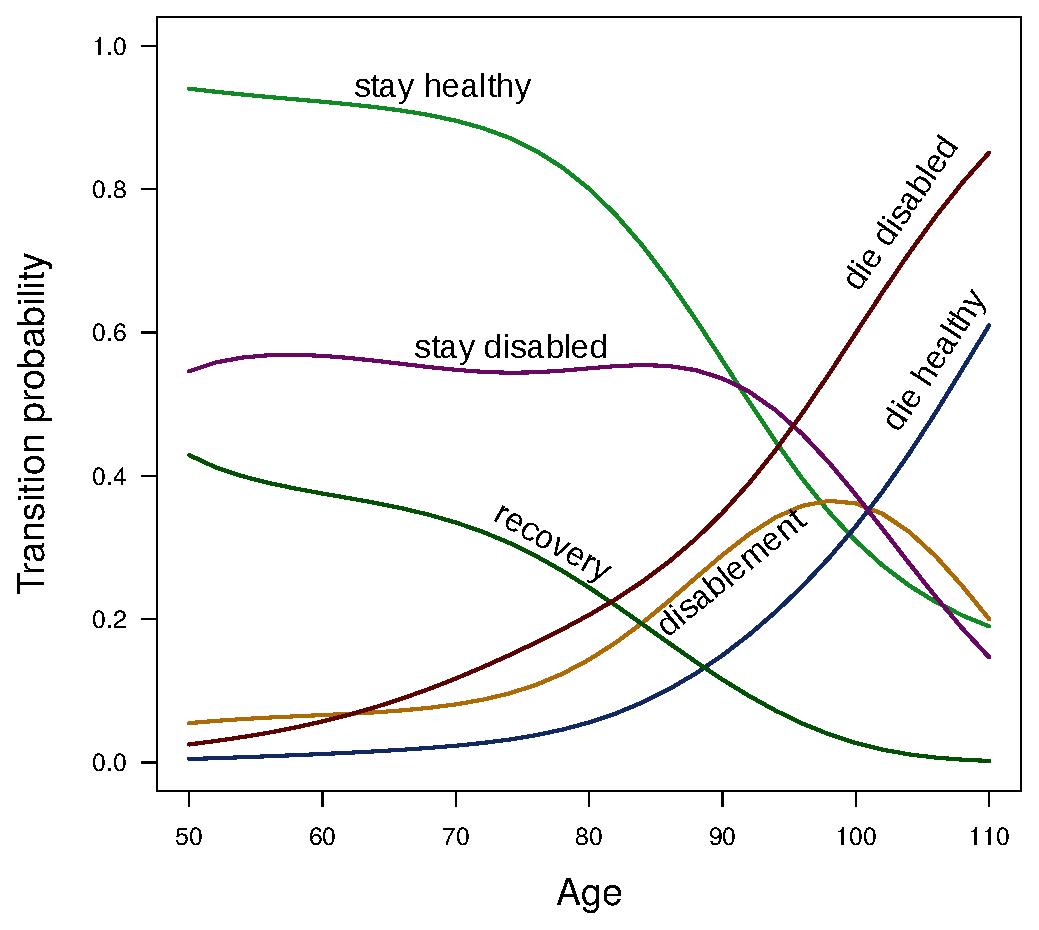
\includegraphics[scale=.7]{Figures/TransitionsInk.pdf}
\caption{Transition probabilities for US females in 2006, as estimated from HRS data, all education groups combined. These age schedules correspond to the arrows in Fig.~\ref{fig:statespace}.}
\end{figure}

The total life expectancies we calculate using HRS data for all education groups combined (and controlling for race and ethnic composition) are very close to the HMD levels and trends, which were based on more aggregate data (See Fig.~\ref{fig:e50}). This gives some assurance that the data and model are working as expected, but one ought not expect the two trends to coincide as a matter of definition: the HRS estimates refer to a statistical centroid of race/ethnicity and education groups, with prevalence having arrived at its steady state given the HRS transition probabilities: the real world underlying HMD estimates is a messy composition and it is not in a steady state, and so we expect some departures, even under perfect data conditions. Also of interest to our study is the size of the educational gradient: we observe an approximately 6-year gap between the highest and lowest educated, which has been increasing for both males and females. This gap size is roughly consistent with \citet{montez2014cumulative}, whose model differs from our own in several ways.

\begin{figure}[ht!]
\centering
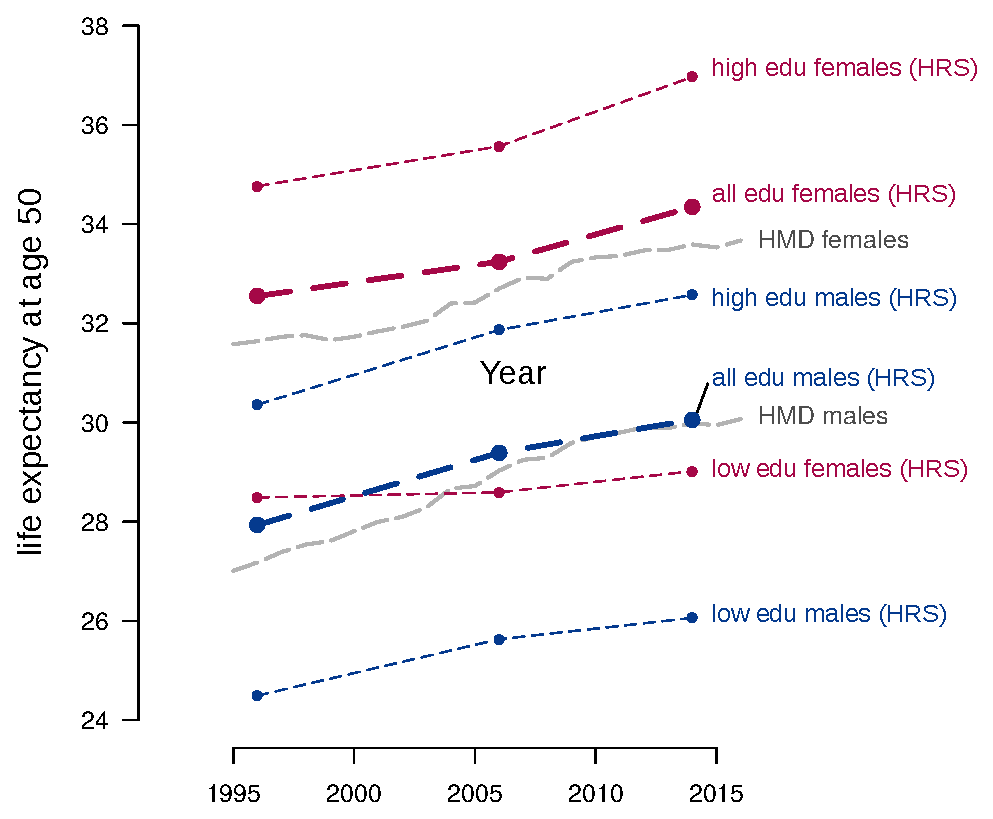
\includegraphics[scale=.7]{Figures/e50_Ink.pdf}
\caption{Life expectancy at age 50 for males (blue) and females (purple) using HRS transition probabilities. Bold dashed lines indicate the HRS estimate for all educational groups combined. It is quite close to the HMD estimate (gray background lines). High education (low education) groups in light dashed lines have approximately three years higher (lower) values than the average for both males and females.}
\label{fig:e50}
\end{figure}

\subsection{Life expectancy with and without disability}

Life expectancy breaks down into two additive expectancies, DFLE and DLE, which we show in Fig.~\ref{fig:barsmales} for males and in Fig.~\ref{fig:barsfemales} for females. We show the breakdown for all education groups blended (Fig.~\ref{fig:barsmalesa} and ~\ref{fig:barsfemalesa}), where the total length of each bar corresponds to the bold dashed point estimates in Fig.~\ref{fig:e50}. Males DFLE increased from 1996 to 2006 to 2014. For females DFLE increased by more than a year in the first period, but stagnated in the second period, even falling by 10 months in the low educated group. DLE held constant for males on the whole, increasing three months for the low-educated. DLE first decreased from 1996 to 2006 then increased by 2014 for an overall increase of 7-8 months in disability over all education groups and females on the whole.  

The fraction of life expectancy at age 50 in the state of disability was decreased by less than a percentage point for males in each education group from 1996 to 2014, and increased by 1-2 percentage points for females. Sex differences are also as expected from the literature: DFLE is 10-20\%, and DLE is 20-40\% higher for females than for males within each year and education group. Notably, most of the increase in LE for females from 2006 to 2014 was due to a 0.98 year increase in DLE (all education groups blended). 

\begin{figure}[ht!]
    \centering
    \begin{subfigure}[b]{0.2\textwidth}
        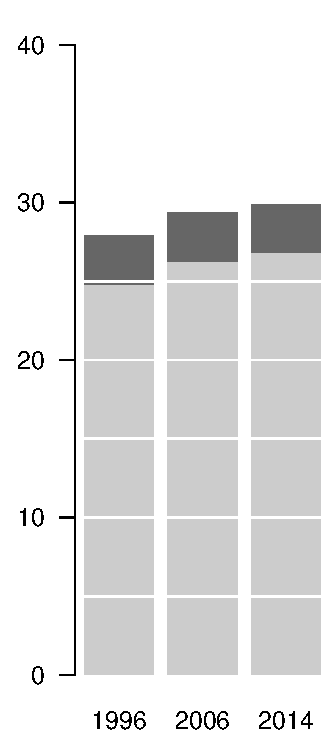
\includegraphics[scale=.5]{Figures/bar_male_all.pdf}
        \caption{All education}
        \label{fig:barsmalesa}
    \end{subfigure}
    ~ %add desired spacing between images, e. g. ~, \quad, \qquad, \hfill etc. 
      %(or a blank line to force the subfigure onto a new line)
    \begin{subfigure}[b]{0.2\textwidth}
        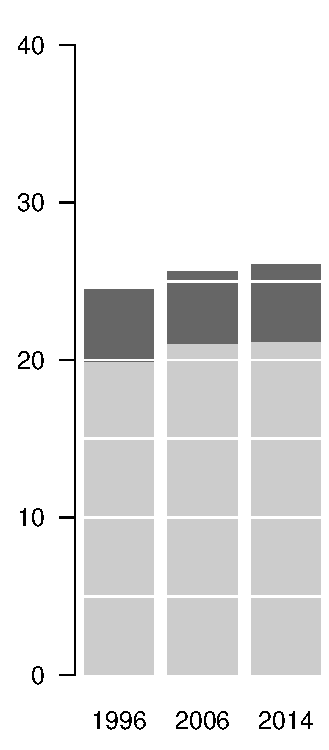
\includegraphics[scale=.5]{Figures/bar_male_pri.pdf}
        \caption{Low education}
    \end{subfigure}
    ~ %add desired spacing between images, e. g. ~, \quad, \qquad, \hfill etc. 
    %(or a blank line to force the subfigure onto a new line)
    \begin{subfigure}[b]{0.2\textwidth}
        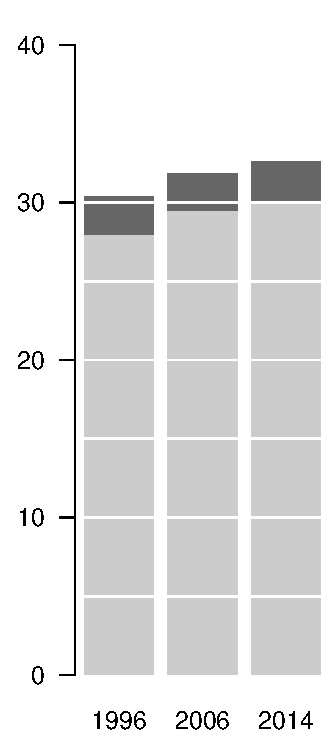
\includegraphics[scale=.5]{Figures/bar_male_uni.pdf}
        \caption{High education}
    \end{subfigure}
    \caption{Male DFLE (light gray) and DLE (dark gray) for all education combined (a), for the low-educated (b) and the high-educated (c) subgroups in 1996, 2006 and 2014. Both DFLE and DLE have increased steadily for each education grouping.}\label{fig:barsmales}
\end{figure}

\begin{figure}[ht!]
    \centering
    \begin{subfigure}[b]{0.2\textwidth}
        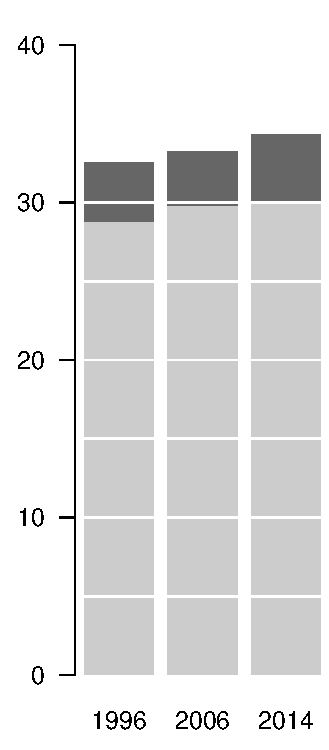
\includegraphics[scale=.5]{Figures/bar_fem_all.pdf}
        \caption{All education}
        \label{fig:barsfemalesa}
    \end{subfigure}
    ~ %add desired spacing between images, e. g. ~, \quad, \qquad, \hfill etc. 
      %(or a blank line to force the subfigure onto a new line)
    \begin{subfigure}[b]{0.2\textwidth}
        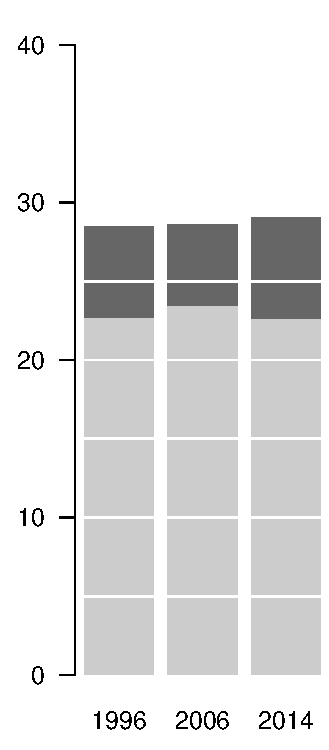
\includegraphics[scale=.5]{Figures/bar_fem_pri.pdf}
        \caption{Low education}
    \end{subfigure}
    ~ %add desired spacing between images, e. g. ~, \quad, \qquad, \hfill etc. 
    %(or a blank line to force the subfigure onto a new line)
    \begin{subfigure}[b]{0.2\textwidth}
        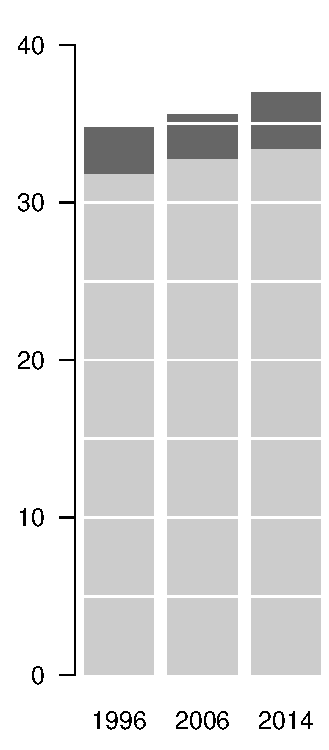
\includegraphics[scale=.5]{Figures/bar_fem_uni.pdf}
        \caption{High education}
        \label{fig:barsfemalesc}
    \end{subfigure}
    \caption{Female DFLE (light gray) and DLE (dark gray) for all education groups blended (a), for the low-educated (b) and the high-educated (c) subgroups in 1996, 2006 and 2014. DFLE has increased for each education group, but DLE was roughly constant, and even decreased slightly over the whole period.}\label{fig:barsfemales}
\end{figure}

\subsection{Decomposition results}
We decompose changes in the values of LE, DFLE, and DLE as represented in Fig.~\ref{fig:barsmalesa}, Fig.~\ref{fig:barsfemalesa}, or the bold dashed line in Fig.~\ref{fig:e50}. To be clear, this quantity is based on blending together education-specific expectancies according to the fraction in each education group at age 50, which also changes over time. The components of change in the value of LE, DFLE, and DLE from 1996 to 2006 and from 2006 to 2014 are summarized in Tab.~\ref{tab:males} and Tab.~\ref{tab:females}, with table shading to indicate the magnitude and direction of effects (green for improvement, purple for deterioration, darker for larger magnitudes). Each cell value has been summed over age. Each table is interpreted as follows: the lower right corner gives the total change in LE for the period, which is the sum of the change in DLE and DFLE (Total margin). The contribution of each transition to each expectancy change is given in the rows labeled Onset (disablement), DF Mortality (disability free), Recovery, and Dis.(abled) Mortality. The effect of changes in disability prevalence at age 50 is given in the \nth{5} row (Age 50 Disab.) and the effect of changes in the education composition is given in the \nth{6} row (Age 50 Educ.). The final row, Total, gives the total change in the given expectancy. The LE gives the marginal row sum, which is identical to decomposing LE directly in the same way (everything is additive).

From Tab. 1a we see that most of the 1.46 year increase in LE was due to improved among those with no disability, adding one year to DFLE and one and a half months to DLE, respectively. In general, mortality improvements in any state contribute to increases in the expectancy of all states. Onset among males improved in both periods, and this adds nearly twice as many years to DFLE as it deducts from DLE. Recovery from disability worsened trivially in the first period, and importantly in the second period, adding one and a half months to DLE and deducting three months from DFLE. We might call the net effect of onset and recovery something like `health dynamics', in which case health dynamics added one and a half months to LE in the first period and deducted one month from LE in the second period. Most change was positive and due to mortality. Had recovery remained unchanged from 2006 to 2014, we might have seen an additional one month increase in LE.

On average, males entering age 50 over the period had a slightly higher prevalence of disability conditional on education group, which deducted less than a month from LE, but this was more than offset by compositional change in the educational attainment of 50-year-olds over the period, which itself added a month to LE in both the first and the second periods. Hypotetically and all else equal, a cohort of 50-year-old males with one half of its members having attained a high school equivalent and the other half with a university degree would have added a further 10 months to LE.

\begin{table}[!ht]
      \caption{Males. Contributions of changes in each transition, disability prevalence at age 50, and the education composition at age 50 to the change in DFLE, DLE, and LE (year units).}
      \label{tab:males}
      \centering
\subfloat[][1996-2006]{
      \begin{tabular}{rrr|r}
      % latex table generated in R 3.5.1 by xtable 1.8-3 package
% Wed Sep 19 13:33:03 2018
 & DFLE & DLE & LE \\ 
  \midrule
Disablement & \cellcolor[HTML]{CEEBC8}{\color[HTML]{000000}0.31} & \cellcolor[HTML]{EEE4EF}{\color[HTML]{000000}-0.18} & \cellcolor[HTML]{E7F3E4}{\color[HTML]{000000}0.13} \\ 
  DF Mortality & \cellcolor[HTML]{358C46}{\color[HTML]{FFFFFF}1.00} & \cellcolor[HTML]{E7F3E4}{\color[HTML]{000000}0.12} & \cellcolor[HTML]{1D7938}{\color[HTML]{FFFFFF}1.12} \\ 
  Recovery & \cellcolor[HTML]{F4F0F4}{\color[HTML]{000000}-0.04} & \cellcolor[HTML]{F1F5F0}{\color[HTML]{000000}0.03} & \cellcolor[HTML]{F4F0F4}{\color[HTML]{000000}-0.01} \\ 
  Dis. Mortality & \cellcolor[HTML]{E7F3E4}{\color[HTML]{000000}0.12} & \cellcolor[HTML]{F1F5F0}{\color[HTML]{000000}0.03} & \cellcolor[HTML]{E7F3E4}{\color[HTML]{000000}0.14} \\ 
   \midrule
Age 50 Disab. & \cellcolor[HTML]{F4F0F4}{\color[HTML]{000000}-0.03} & \cellcolor[HTML]{F1F5F0}{\color[HTML]{000000}0.01} & \cellcolor[HTML]{F4F0F4}{\color[HTML]{000000}-0.02} \\ 
  Age 50 Educ. & \cellcolor[HTML]{E7F3E4}{\color[HTML]{000000}0.13} & \cellcolor[HTML]{F4F0F4}{\color[HTML]{000000}-0.03} & \cellcolor[HTML]{F1F5F0}{\color[HTML]{000000}0.09} \\ 
   \midrule
Total & \cellcolor[HTML]{00441A}{\color[HTML]{FFFFFF}1.49} & \cellcolor[HTML]{F4F0F4}{\color[HTML]{000000}-0.03} & \cellcolor[HTML]{00441A}{\color[HTML]{FFFFFF}1.46} \\ 
  
     \end{tabular}
}
~
\subfloat[][2006-2014]{
      \begin{tabular}{rrr|r}
      % latex table generated in R 3.5.1 by xtable 1.8-3 package
% Wed Sep 19 13:33:04 2018
 & DFLE & DLE & LE \\ 
  \midrule
Disablement & \cellcolor[HTML]{E7F3E4}{\color[HTML]{000000}0.15} & \cellcolor[HTML]{F4F0F4}{\color[HTML]{000000}-0.09} & \cellcolor[HTML]{F1F5F0}{\color[HTML]{000000}0.06} \\ 
  DF Mortality & \cellcolor[HTML]{ABDDA5}{\color[HTML]{000000}0.52} & \cellcolor[HTML]{F1F5F0}{\color[HTML]{000000}0.06} & \cellcolor[HTML]{ABDDA5}{\color[HTML]{000000}0.58} \\ 
  Recovery & \cellcolor[HTML]{E9D8EA}{\color[HTML]{000000}-0.26} & \cellcolor[HTML]{E7F3E4}{\color[HTML]{000000}0.13} & \cellcolor[HTML]{EEE4EF}{\color[HTML]{000000}-0.13} \\ 
  Dis. Mortality & \cellcolor[HTML]{F1F5F0}{\color[HTML]{000000}0.09} & \cellcolor[HTML]{F1F5F0}{\color[HTML]{000000}0.03} & \cellcolor[HTML]{E7F3E4}{\color[HTML]{000000}0.12} \\ 
   \midrule
Age 50 Disab. & \cellcolor[HTML]{F4F0F4}{\color[HTML]{000000}-0.05} & \cellcolor[HTML]{F1F5F0}{\color[HTML]{000000}0.02} & \cellcolor[HTML]{F4F0F4}{\color[HTML]{000000}-0.04} \\ 
  Age 50 Educ. & \cellcolor[HTML]{F1F5F0}{\color[HTML]{000000}0.09} & \cellcolor[HTML]{F4F0F4}{\color[HTML]{000000}-0.02} & \cellcolor[HTML]{F1F5F0}{\color[HTML]{000000}0.07} \\ 
   \midrule
Total & \cellcolor[HTML]{ABDDA5}{\color[HTML]{000000}0.54} & \cellcolor[HTML]{E7F3E4}{\color[HTML]{000000}0.12} & \cellcolor[HTML]{94D090}{\color[HTML]{000000}0.67} \\ 
  
     \end{tabular}
}
\end{table}

\begin{table}[!ht]
      \caption{Females. Contributions of changes in each transition, disability prevalence at age 50, and the education composition at age 50 to the change in DFLE, DLE, and LE (year units).}}
      \label{tab:females}
      \centering
\subfloat[][1996-2006]{
      \begin{tabular}{rrr|r}
      % latex table generated in R 3.5.1 by xtable 1.8-3 package
% Wed Sep 19 13:33:03 2018
 & DFLE & DLE & LE \\ 
  \midrule
Onset & \cellcolor[HTML]{ABDDA5}{\color[HTML]{000000}0.59} & \cellcolor[HTML]{DFCAE2}{\color[HTML]{000000}-0.34} & \cellcolor[HTML]{DDF1D7}{\color[HTML]{000000}0.26} \\ 
  DF Mortality & \cellcolor[HTML]{7AC07A}{\color[HTML]{000000}0.76} & \cellcolor[HTML]{F1F5F0}{\color[HTML]{000000}0.09} & \cellcolor[HTML]{5FB165}{\color[HTML]{FFFFFF}0.85} \\ 
  Recovery & \cellcolor[HTML]{F1F5F0}{\color[HTML]{000000}0.07} & \cellcolor[HTML]{F4F0F4}{\color[HTML]{000000}-0.01} & \cellcolor[HTML]{F1F5F0}{\color[HTML]{000000}0.06} \\ 
  Dis. Mortality & \cellcolor[HTML]{DFCAE2}{\color[HTML]{000000}-0.39} & \cellcolor[HTML]{F4F0F4}{\color[HTML]{000000}-0.08} & \cellcolor[HTML]{D2B9DA}{\color[HTML]{000000}-0.47} \\ 
   \midrule
Age 50 Disab. & \cellcolor[HTML]{EEE4EF}{\color[HTML]{000000}-0.14} & \cellcolor[HTML]{F1F5F0}{\color[HTML]{000000}0.05} & \cellcolor[HTML]{F4F0F4}{\color[HTML]{000000}-0.09} \\ 
  Age 50 Educ. & \cellcolor[HTML]{F1F5F0}{\color[HTML]{000000}0.09} & \cellcolor[HTML]{F4F0F4}{\color[HTML]{000000}-0.01} & \cellcolor[HTML]{F1F5F0}{\color[HTML]{000000}0.08} \\ 
   \midrule
Total & \cellcolor[HTML]{499E55}{\color[HTML]{FFFFFF}0.99} & \cellcolor[HTML]{E9D8EA}{\color[HTML]{000000}-0.30} & \cellcolor[HTML]{94D090}{\color[HTML]{000000}0.69} \\ 
  
     \end{tabular}
}
~
\subfloat[][2006-2014]{
      \begin{tabular}{rrr|r}
      % latex table generated in R 3.5.1 by xtable 1.8-3 package
% Wed Sep 19 13:33:03 2018
 & DFLE & DLE & LE \\ 
  \midrule
Onset & \cellcolor[HTML]{F4F0F4}{\color[HTML]{000000}-0.00} & \cellcolor[HTML]{F4F0F4}{\color[HTML]{000000}-0.01} & \cellcolor[HTML]{F4F0F4}{\color[HTML]{000000}-0.02} \\ 
  DF Mortality & \cellcolor[HTML]{12672E}{\color[HTML]{FFFFFF}1.21} & \cellcolor[HTML]{E7F3E4}{\color[HTML]{000000}0.15} & \cellcolor[HTML]{075524}{\color[HTML]{FFFFFF}1.36} \\ 
  Recovery & \cellcolor[HTML]{834692}{\color[HTML]{FFFFFF}-1.04} & \cellcolor[HTML]{94D090}{\color[HTML]{000000}0.62} & \cellcolor[HTML]{D2B9DA}{\color[HTML]{000000}-0.42} \\ 
  Dis. Mortality & \cellcolor[HTML]{CEEBC8}{\color[HTML]{000000}0.38} & \cellcolor[HTML]{F1F5F0}{\color[HTML]{000000}0.08} & \cellcolor[HTML]{BDE4B6}{\color[HTML]{000000}0.45} \\ 
   \midrule
Age 50 Disab. & \cellcolor[HTML]{E9D8EA}{\color[HTML]{000000}-0.29} & \cellcolor[HTML]{E7F3E4}{\color[HTML]{000000}0.10} & \cellcolor[HTML]{EEE4EF}{\color[HTML]{000000}-0.19} \\ 
  Age 50 Educ. & \cellcolor[HTML]{EEE4EF}{\color[HTML]{000000}-0.14} & \cellcolor[HTML]{F1F5F0}{\color[HTML]{000000}0.05} & \cellcolor[HTML]{F4F0F4}{\color[HTML]{000000}-0.09} \\ 
   \midrule
Total & \cellcolor[HTML]{E7F3E4}{\color[HTML]{000000}0.12} & \cellcolor[HTML]{499E55}{\color[HTML]{FFFFFF}0.98} & \cellcolor[HTML]{1D7938}{\color[HTML]{FFFFFF}1.10} \\ 
  
     \end{tabular}
}
\end{table}

Trends for females have also been dominated by mortality improvements of the non-disabled, adding ten months to LE in the first period and 1.36 years in the second period, most of which accrued to DFLE. Mortality of the disabled population deteriorated in the first period and recovered in the second period, for a net zero increase LE over the whole period. Onset improved in the first period, deducting four months from DLE and adding seven months to DFLE. In the second period onset stagnated, and more importantly recovery deteriorated so much as to add seven months to DLE and deduct over a year from DFLE. In the net, health dynamics worsened slightly from 1996 to 2014, deducting one and a half from LE. Most of the improvement in female life expectancy at age 50 in the second period was due to increased DLE, making this a period of disability expansion, driven entirely by a setback in recovery from disability. All else equal, had recovery rates over age 50 remained unchanged for females from 2006 to 2014, LE could have increased by a further five months, DLE would have only increased by four months, and DFLE by over a year. 

The fraction of 50-year old females with at least one ADL has increased over the whole period, leading to deductions from DFLE and LE, and a total of two months of increase in DLE. That is, 50-years are getting off to a worse start, all else equal. In the first period this was offset entirely by educational expansion interacting with the educational gradient in health in mortality. The effect of education unexpectedly turned negative in the second period-- this is counter to our intuition, and we will investigate this at length before this work is finalized. Hypothetically and all else equal, a cohort of 50-year-old females with one half of its members having attained a high school equivalent and the other half with a university degree would have added a further 1.58 years to LE.

\section{Discussion}
\label{sec:discussion}
Life expectancy has been improving, but not as fast as it could have been. Our decomposition results show that disability and education-specific mortality has for the most part been a positive driver of mortality change, and this includes even mortality improvements among the disabled. For females since 2006 mortality improvement among those with at least one ADL added almost five times more years to DFLE than to DLE (see Tab.~2b), a positive finding which may run counter to intuition. Mortality change among those with no reported ADL has been a consistently positive driver of improvement in DFLE. Some of these added years of life inevitably spill over into DLE, but this is a relatively small externality, and it has not been a driver of disability expansion as some might fear. Recovery from disability presents a more worrying trend since 2006 for both sexes, but especially females. Based on our decomposition it is also an obvious opportunity for intervention, and an often overlooked lever for disability change, since reduced or delayed disability onset also reduces the need for active recovery. Delaying onset is always an effective option to reduce DLE and increase DFLE \citep[c.f.][]{freedman2016disability}, but rates of transition into disability are presently high enough to merit population-level research into recovery in more detail than what we can provide in this analysis.

Compositional change has been only a minor driver of 50+ mortality change in the United States over the past 20 years, but this will surely change in the coming decades as more educated cohorts enter into old age. SES differences in disability and mortality in the United States are wide and getting wider \citep{montez2014cumulative}. Aim aim of public health is to narrow this gap, and one way to narrow the gap is to shift everyone toward the lower risk set, which in our analysis is the high education group. This trend has been happening in older ages and we expect it will continue to do so in the United States, just as it will with other countries \citep{kc2010projection}. We are rather worried about patterns of disease and disability that happen \emph{below} age 50 (and which we do not detect in this study), especially contemporary obesity patterns among adults \citep{flegal2012prevalence}. Obesity acts to increase the fraction of old age spent in disability by getting off to a bad start \citep{alley2007changing}, and they may be a driver of the worsening in the probability of recovering from disability \citep[c.f.,][]{walter2009mortality}. We urge common sense measures today to reduce the risk factors of obesity, which is and will increasingly become a primary driver of disability and length of life in old ages \citep{mehta2017population}.

From 1996 to 2006 we find that the fraction of life after 50 spent with a disability decreased unequivocally for both males and females, and this continued to decline for males after 2006, as females had a setback in disability dynamics. 

On the whole, our decomposition results show that over the 19 years from 1996 to 2014 net health dynamics worked to keep disabled life expectancy in dynamic equilibrium for males, consistent with \citet{manton1982changing} and others. Females have shown a more worrying trend over the period studied, with worsened recovery from disability since 2006 acting to decrease life expectancy and increase both absolute and relative time spent disabled. Disability expansion occurred for females over the whole period studied due primarily to changes in health dynamics (onset and recovery), which acted to deduct four months from DLE from 1996 to 2006, and then add seven months to DLE from 2006 to 2014. Female mortality deterioration of the disabled population in the first period was offset by mortality improvements in the second period, leaving the final net increase in DLE from 1996 to 2014 almost entirely due to mortality improvements of the non-disabled population. Mortality improvements are unequivocally good, whether they lead to disability expansion or compression, and in our case they have had a neutral effect on disability compression. The best levers for interventions with respect to the time and fraction of life spent disabled are those that influence onset and recovery of disability.

Our study is the first to demographically decompose a multistate health model of these dimensions, in a way that intuitively partitions observed changes in LE, DFLE, and DLE into additive components that appeal to understanding a simple process model of disablement. Our results highlight key areas for intervention (recovery, onset, and disability before old age) and demystify the US lag in world life expectancy rankings (see Fig.~\ref{fig:uslose}). The culprits of US life expectancy lag at age 50 are distributed:\footnote{\rd{NOTE} We will aim to quantify these `culprits' in a more meaningful way moving forward, possibly doing a redux of Fig.~\ref{fig:uslose} with a counter-factual US trend.}

\begin{enumerate}
\item The large SES gradients in health and mortality, especially the injurious effects of the lower tail of this distribution.
\item The worsened disability dynamics of the 50+ population, which could have added half a year to LE for females, had they remained unchanged since 2006. Although disability dynamics have had no effect on male LE in the net, they remain an available lever to improve LE.
\item The 50+ population is getting off to a worse start in disability prevalence, net of educational change.
\end{enumerate}

Secular mortality change, net of everything included in our simple model (three education states, two disability states) is not the culprit of laggard improvement in the US: Disability-free mortality has been improving just as it should, and its effects on the fraction of life spent disabled have been neutral or positive. The mortality of those with one or more disabilities has evolved inconsistently, but note that for males over the entire period its improvements added more years to DFLE than they did to DLE. Forthcoming changes in the health and SES composition of the renewing 50+ population will to some degree offset each other, as the fruits of past educational expansion arrive in old age, with the extra baggage of higher fractions disabled.

\subsection{Plain language limitations}
This study is not perfect, but we think it sends a clear message that is empirically sound. Some things we can not solve or do not handle are: i) Due to the HRS survey wave spacing short spells of disability are likely to go unrecorded, and so these do not enter into our transition probability structure, thereby potentially biasing our results. ii) Our Markov state space is not a very good articulation of the process of disablement. For example, we could account for stages of severity rather than simply counting ADLs. iii) We do not explicitly account for risk factors such as obesity, chronic illness, or lifecourse characteristics that are known to co-vary with health. iv) Recovery may be duration dependent and not just age dependent. v) Survey attrition is probably selective in such a way as to bias our transition probabilities, although we may account for this moving forward. Rather than accounting for each of these things we work to get the best possible specification of our stated model, which in any case is a decent approximation of the world. While Sullivan-based measures are robust to a certain extent to model mis-specification (they are process free), these tell us nothing about state-specific mortality trends or the process of entry and exit from disablement, nor the effects of population composition in the age of left-truncation (50 in our case), and they are a lagged result of health dynamics rather than a real-time snapshot. These are items we think make up the primary value of our study. Also multistate Markov models are more flexible than they get credit for.

\section{Conclusions}
The United states has been a laggard in life expectancy at age 50, but there are some drivers that are ripe for intervention. Secular mortality change, net of health dynamics and population composition, has been a primary driver of mean time spent free of and in disability. Mortality improvements do not lead to disability expansion. Potential improvement in disability recovery rates is a strong and under-recognized lever to both increase overall life expectancy and shift years lived in disability to good health. Recovery will remain a lever as long as the transition rate into disability is high, in part because mortality rates of the disabled have been and will probably continue falling. Investment in recovery is not to the exclusion of actions that would delay or avoid onset, which are far more effective. Life expectancy improvement at age 50 from educational expansion has been modest in the period studied, but holds much potential to fuel further increases in life expectancy for both males and females. While education will be a positive force, the trend of increased rates of disability among those entering old age is worrisome, and we suspect that it is being driven by obesity. The obesity epidemic of today will have echoes in old-age disability patterns for decades to come if the population in young and middle ages does not stem the onset of obesity and take steps to reduce its severity. Obesity, in part via disability, will contribute to a continuance of US laggard status in old-age life expectancy.  

%\section{Conclusions}
%\label{sec:conclusions}
% bibliography
\bibliographystyle{spbasic}
\bibliography{references}  
\end{document}
